\documentclass[12pt]{article}%
\usepackage{amsfonts}
\usepackage{fancyhdr}
\usepackage[a4paper, top=2.5cm, bottom=2.5cm, left=2.2cm, right=2.2cm]%
{geometry}
\usepackage{times}
\usepackage{listings}
\usepackage{amsmath}
\usepackage{amssymb}
\usepackage{graphicx}%
\setcounter{MaxMatrixCols}{30}
\newtheorem{theorem}{Theorem}
\newtheorem{acknowledgement}[theorem]{Acknowledgement}
\newtheorem{algorithm}[theorem]{Algorithm}
\newtheorem{axiom}{Axiom}
\newtheorem{case}[theorem]{Case}
\newtheorem{claim}[theorem]{Claim}
\newtheorem{conclusion}[theorem]{Conclusion}
\newtheorem{condition}[theorem]{Condition}
\newtheorem{conjecture}[theorem]{Conjecture}
\newtheorem{corollary}[theorem]{Corollary}
\newtheorem{criterion}[theorem]{Criterion}
\newtheorem{definition}[theorem]{Definition}
\newtheorem{example}[theorem]{Example}
\newtheorem{exercise}[theorem]{Exercise}
\newtheorem{lemma}[theorem]{Lemma}
\newtheorem{notation}[theorem]{Notation}
\newtheorem{problem}[theorem]{Problem}
\newtheorem{proposition}[theorem]{Proposition}
\newtheorem{remark}[theorem]{Remark}
\newtheorem{solution}[theorem]{Solution}
\newtheorem{summary}[theorem]{Summary}
\newenvironment{proof}[1][Proof]{\textbf{#1.} }{\ \rule{0.5em}{0.5em}}
\usepackage{graphicx}
\graphicspath{ {/Users/dkishan/Desktop/FirstSemUB/ComputerSecurity/hw3/} }
\newcommand{\Q}{\mathbb{Q}}
\newcommand{\R}{\mathbb{R}}
\newcommand{\C}{\mathbb{C}}
\newcommand{\Z}{\mathbb{Z}}

\begin{document}

\title{Computer Security Homework-1}
\author{Kishan Dhamotharan}
\date{\today}
\maketitle
\begin{center}
 Person \# 50287619
\end{center}
\section{Problem 1}

Programming Language used: Python 3\newline
Imports/Libraries used: pycryptodome, matplotlib\newline
Commands to install dependences:\newline
- sudo pip install pycryptodome\newline
- sudo pip install pycryptodomex\newline
Additional(Graph can be commented out):\newline
$https://matplotlib.org/faq/installing_faq.html$\newline
- python -mpip install matplotlib \newline
References
$https://pycryptodome.readthedocs.io/en$\newline
Ran on virtual machine.

\subsection{Solution (a)}
\begin{lstlisting}[language=Python]
import os, random, struct
from Crypto.Cipher import AES
from Crypto.Random import get_random_bytes
from timeit import default_timer as timer
import matplotlib.pyplot as plt
#Key Generation
start_key=timer()
key = get_random_bytes(16)
end_key=timer()
iv = get_random_bytes(16)
aes = AES.new(key, AES.MODE_CBC, iv)
read_size = 512
def get_time_per_byte(capture_time):
    return [capture_time[0]/(1024*1024), capture_time[1]/(1024*1024),
            capture_time[2]/(1024),capture_time[3]/(1024)]


def encrypt(input_file, enc_file):
    file_size = os.path.getsize(input_file)
    t_time=0
    with open(enc_file, 'wb') as fout:
        fout.write(struct.pack('<Q', file_size))
        fout.write(iv)
        with open(input_file, 'rb') as fin:
            while True:
                data = fin.read(read_size)
                n = len(data)
                if n == 0:
                    break
                elif n % 16 != 0:
                    data += ' ' * (16 - n % 16) #
                start = timer()
                encrypted_data = aes.encrypt(data)
                end = timer()
                t_time+=(end-start)
                fout.write(encrypted_data)
    return t_time

def decrypt(enc_file, verification_file):
    t_time=0
    with open(enc_file, 'rb') as fin:
        file_size = struct.unpack('<Q', fin.read(struct.calcsize('<Q')))[0]
        iv = fin.read(16)
        aes = AES.new(key, AES.MODE_CBC, iv)
        with open(verification_file, 'wb') as fout:
            while True:
                data = fin.read(read_size)
                n = len(data)
                if n == 0:
                    break
                start = timer()
                decrpted_data = aes.decrypt(data)
                end = timer()
                t_time+=(end-start)
                n = len(decrpted_data)
                if file_size > n:
                    fout.write(decrpted_data)
                else:
                    fout.write(decrpted_data[:file_size]) # <- remove padding on last block
                file_size -= n
    return t_time
input_files=['bigfile.txt', 'smallfile.txt']
enc_files=['q1aAnsBigFile.enc', 'q1aAnsSmallFile.enc']
verification_files=['q1aVeriBigFile.txt', 'q1aVeriSmallFile.enc']
capture_time=[]
for i in range(2):
    capture_time.append(encrypt(input_files[i], enc_files[i]))
    capture_time.append(decrypt(enc_files[i], verification_files[i]))

plt.plot(capture_time[:2], label='1 MB file')
plt.plot(capture_time[2:4], dashes=[6, 2], label='1 KB file')
plt.xticks(range(2), ['Encryption','Decryption'])
plt.ylabel('time(s)')
plt.grid(axis='y', linestyle='-')
plt.legend()
plt.savefig('q1a.png')
time_per_byte=get_time_per_byte(capture_time)
print('Total time')
print('Encryption -  1MB: %E, 1KB: %E' %(capture_time[0], capture_time[2]))
print('Decryption -  1MB: %E, 1KB: %E' %(capture_time[1], capture_time[3]))
print('Per Byte')
print('Encryption -  1MB: %E, 1KB: %E' %(time_per_byte[0], time_per_byte[2]))
print('Decryption -  1MB: %E, 1KB: %E' %(time_per_byte[1], time_per_byte[3]))
print('Key Gen')
print('Time: %E' %(end_key-start_key))
\end{lstlisting}
\begin{tabular}{ |p{8cm}|p{3cm}|p{3cm}|p{3cm} }
 \hline
 \multicolumn{3}{|c|}{AES 128 CBC} \\
 \hline
	 & 1MB file & 1KB file\\
 \hline
 Time taken for full file Encryption   &   2.140892E-02   &  7.137400E-05 \\
  \hline
 Time taken for full file Decryption &  1.459782E-02  & 3.848004E-05	\\
 \hline
 Time taken per byte Encryption   &  2.041714E-08    & 6.970117E-08  \\
  \hline
 Time taken per byte Decryption & 1.392157E-08   & 3.757816E-08	\\
 \hline
 Time taken for key generation &   1.399399E-05  & 	\\
 \hline
\end{tabular}
\begin{figure}[h]
    \centering
	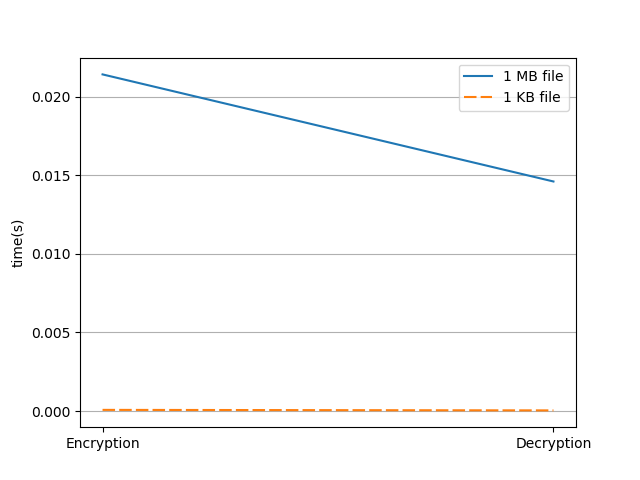
\includegraphics[scale=0.5]{q1a}
\end{figure}
 
Observation:
In CBC mode it can be observed that decryption happens a little faster than the encryption, this is a expected behavior as encryption of CBC happens only sequentially, that is encrypt 1st block, then 2nd and so on. Whereas, decryption can happen in parallel as p[1] = c[0] XOR decrypt(c[1]), it does not depend on the p[0], hence can be completely parrelized.

\subsection{Solution (b)}
\begin{lstlisting}[language=Python]
from Crypto.Cipher import AES
from Crypto.Util import Counter
from Crypto import Random
import matplotlib.pyplot as plt
from timeit import default_timer as timer

#Key Generation
nonce = Random.get_random_bytes(8)
count = Counter.new(64, nonce)
start_key=timer()
key = Random.get_random_bytes(16)
end_key=timer()

def get_time_per_byte(capture_time):
    return [capture_time[0]/(1024*1024), capture_time[1]/(1024*1024),
            capture_time[2]/(1024),capture_time[3]/(1024)]

def encrypt(input_file, enc_file):
    encrypt = AES.new(key, AES.MODE_CTR, counter=count)
    with open(enc_file, 'wb') as fout:
        with open(input_file, 'rb') as fin:
            data = fin.read()
            start = timer()
            encrypted = encrypt.encrypt(data)
            end = timer()
            fout.write(encrypted)
    return(end-start)
    
def decrypt(enc_file, verification_file):
    count = Counter.new(64, nonce)
    decrypt = AES.new(key, AES.MODE_CTR, counter=count)
    with open(enc_file, 'rb') as fin:
        with open(verification_file, 'wb') as fout:
            data = fin.read()
            start = timer()
            decrypted = decrypt.decrypt(data)
            end = timer()
            fout.write(decrypted)
    return(end-start)
input_files=['bigfile.txt', 'smallfile.txt']
enc_files=['q1bAnsBigFile.enc', 'q1bAnsSmallFile.enc']
verification_files=['q1bVeriBigFile.txt', 'q1bVeriSmallFile.enc']
capture_time=[]
for i in range(2):
    capture_time.append(encrypt(input_files[i], enc_files[i]))
    capture_time.append(decrypt(enc_files[i], verification_files[i]))

plt.plot(capture_time[:2], label='1 MB file')
plt.plot(capture_time[2:4], dashes=[6, 2], label='1 KB file')
plt.xticks(range(2), ['Encryption','Decryption'])
plt.ylabel('time(s)')
plt.grid(axis='y', linestyle='-')
plt.legend()
plt.savefig('q1b.png')
time_per_byte=get_time_per_byte(capture_time)
print('Total time')
print('Encryption -  1MB: %E, 1KB: %E' %(capture_time[0], capture_time[2]))
print('Decryption -  1MB: %E, 1KB: %E' %(capture_time[1], capture_time[3]))
print('Per Byte')
print('Encryption -  1MB: %E, 1KB: %E' %(time_per_byte[0], time_per_byte[2]))
print('Decryption -  1MB: %E, 1KB: %E' %(time_per_byte[1], time_per_byte[3]))
print('Key Gen')
print('Time: %E' %(end_key-start_key))
\end{lstlisting}
\begin{tabular}{ |p{8cm}|p{3cm}|p{3cm}|p{3cm} }
 \hline
 \multicolumn{3}{|c|}{AES 128 CTR} \\
 \hline
	 & 1MB file & 1KB file\\
 \hline
 Time taken for full file Encryption   & 6.125177E-03    & 7.298501E-05  \\
  \hline
 Time taken for full file Decryption &  3.028722E-03  &  3.369001E-05	\\
 \hline
 Time taken per byte Encryption   & 5.841424E-09    &  7.127443E-08 \\
  \hline
 Time taken per byte Decryption & 2.888414E-09  & 	3.290040E-08\\
 \hline
 Time taken for key generation &  9.277021E-06  & 	\\
 \hline
\end{tabular}
\begin{figure}[h]
    \centering
	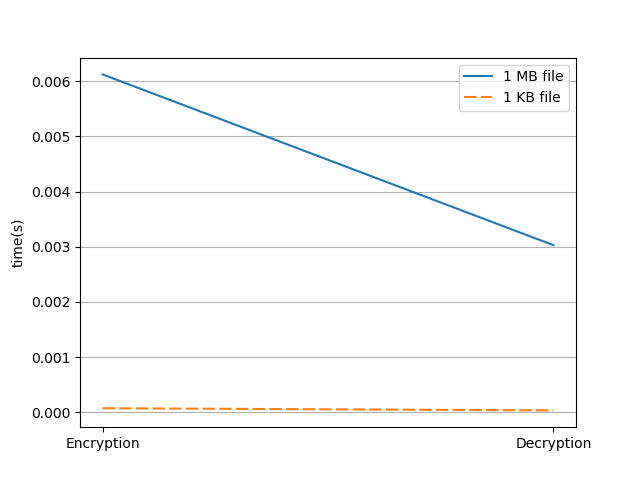
\includegraphics[scale=0.5]{q1b}
\end{figure}

Observation: CTR mode is much faster than the CBC mode as it is parallelized on both encryption and decryption. So, As expected we can see the significant improvement between them.

\subsection{Solution (c)}
\begin{lstlisting}[language=Python]
from Crypto.Cipher import AES
from Crypto.Util import Counter
from Crypto import Random
import matplotlib.pyplot as plt
from timeit import default_timer as timer

#Key Generation
nonce = Random.get_random_bytes(8)
count = Counter.new(64, nonce)
start_key=timer()
key = Random.get_random_bytes(32)
end_key=timer()

def get_time_per_byte(capture_time):
    return [capture_time[0]/(1024*1024), capture_time[1]/(1024*1024),
            capture_time[2]/(1024),capture_time[3]/(1024)]

#Encryption
def encrypt(input_file, enc_file):
    encrypt = AES.new(key, AES.MODE_CTR, counter=count)
    with open(enc_file, 'wb') as fout:
        with open(input_file, 'rb') as fin:
            data = fin.read()
            start = timer()
            encrypted = encrypt.encrypt(data)
            end = timer()
            fout.write(encrypted)
    return(end-start)
    
 #Decryption  
def decrypt(enc_file, verification_file):
    count = Counter.new(64, nonce)
    decrypt = AES.new(key, AES.MODE_CTR, counter=count)
    with open(enc_file, 'rb') as fin:
        with open(verification_file, 'wb') as fout:
            data = fin.read()
            start = timer()
            decrypted = decrypt.decrypt(data)
            end = timer()
            fout.write(decrypted)
    return(end-start)

input_files=['bigfile.txt', 'smallfile.txt']
enc_files=['q1cAnsBigFile.enc', 'q1cAnsSmallFile.enc']
verification_files=['q1cVeriBigFile.txt', 'q1cVeriSmallFile.enc']
capture_time=[]
for i in range(2):
    capture_time.append(encrypt(input_files[i], enc_files[i]))
    capture_time.append(decrypt(enc_files[i], verification_files[i]))

plt.plot(capture_time[:2], label='1 MB file')
plt.plot(capture_time[2:4], dashes=[6, 2], label='1 KB file')
plt.xticks(range(2), ['Encryption','Decryption'])
plt.ylabel('time(s)')
plt.grid(axis='y', linestyle='-')
plt.legend()
plt.savefig('q1c.png')
time_per_byte=get_time_per_byte(capture_time)
print('Total time')
print('Encryption -  1MB: %E, 1KB: %E' %(capture_time[0], capture_time[2]))
print('Decryption -  1MB: %E, 1KB: %E' %(capture_time[1], capture_time[3]))
print('Per Byte')
print('Encryption -  1MB: %E, 1KB: %E' %(time_per_byte[0], time_per_byte[2]))
print('Decryption -  1MB: %E, 1KB: %E' %(time_per_byte[1], time_per_byte[3]))
print('Key Gen')
print('Time: %E' %(end_key-start_key))

\end{lstlisting}


\begin{tabular}{ |p{8cm}|p{3cm}|p{3cm}|p{3cm} }
 \hline
 \multicolumn{3}{|c|}{AES 256 CTR} \\
 \hline
	 & 1MB file & 1KB file\\
 \hline
 Time taken for full file Encryption   &   6.155830E-03   & 7.448002E-05  \\
  \hline
 Time taken for full file Decryption & 3.985250E-03   & 6.230804E-05	\\
 \hline
 Time taken per byte Encryption   &  5.870657E-09    & 7.273439E-08  \\
  \hline
 Time taken per byte Decryption & 3.800631E-09  & 6.084770E-08	\\
 \hline
 Time taken for key generation & 1.801801E-05   & 	\\
 \hline
\end{tabular}
\begin{figure}[h]
    \centering
	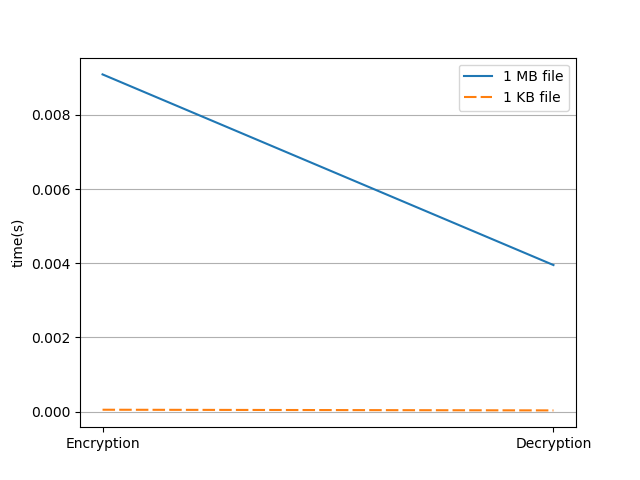
\includegraphics[scale=0.5]{q1c}
\end{figure}

Observation: This is a expected behaviour, as discussed in the lecture, there is a very slight increase in the encryption and decryption time when compared to the CTR 128, reason for this observation is: larger the key size -> more computation time.

\subsection{Solution (d)}
\begin{lstlisting}[language=Python]
from Crypto.Hash import SHA256
from Crypto.Hash import SHA512
from Crypto.Hash import SHA3_256
from timeit import default_timer as timer
import matplotlib.pyplot as plt
import numpy as np
input_files=['smallfile.txt','bigfile.txt']
capture_time=[]

def get_time_per_byte(capture_time):
    return [capture_time[0]/(1024), capture_time[1]/(1024),
            capture_time[2]/(1024),capture_time[3]/(1024*1024),
            capture_time[4]/(1024*1024),capture_time[5]/(1024*1024)]

for input_file in input_files:
    with open(input_file, 'rb') as fin:
        data = fin.read()
        start = timer()
        hash=SHA256.new()
        hash.update(data)
        end = timer()
        print('SHA_256: ', hash.hexdigest())
        capture_time.append(end-start)
    with open(input_file, 'rb') as fin:
        data = fin.read()
        start = timer()
        hash=SHA512.new()
        hash.update(data)
        hash.hexdigest()
        end = timer()
        print('SHA_512: ', hash.hexdigest())
        capture_time.append(end-start)
    with open(input_file, 'rb') as fin:
        start = timer()
        data = fin.read()
        hash=SHA3_256.new()
        hash.update(data)
        end = timer()
        print('SHA3_256: ', hash.hexdigest())
    capture_time.append(end-start)

plt.plot(capture_time[0:3], label='1 KB file')
plt.plot(capture_time[3:6], dashes=[6, 2], label='1 MB file')
plt.xticks(range(3), ['SHA256','SHA512','SHA3_256'])
plt.ylabel('time(s)')
plt.grid(axis='y', linestyle='-')
plt.legend()
plt.savefig('q1d.png')
time_per_byte=get_time_per_byte(capture_time)
print('Total time')
print('SHA256 -  1MB: %E, 1KB: %E' %(capture_time[3], capture_time[0]))
print('SHA_512 -  1MB: %E, 1KB: %E' %(capture_time[4], capture_time[1]))
print('SHA3_256 -  1MB: %E, 1KB: %E' %(capture_time[5], capture_time[2]))
print('Per Byte')
print('SHA256 -  1MB: %E, 1KB: %E' %(time_per_byte[3], time_per_byte[0]))
print('SHA_512 -  1MB: %E, 1KB: %E' %(time_per_byte[4], time_per_byte[1]))
print('SHA3_256 -  1MB: %E, 1KB: %E' %(time_per_byte[5], time_per_byte[2]))

\end{lstlisting}
\begin{tabular}{ |p{8cm}|p{3cm}|p{3cm}|p{3cm} }
 \hline
 \multicolumn{3}{|c|}{Hash Functions} \\
 \hline
	 & 1MB file & 1KB file\\
 \hline
 Time taken for SHA256   &   7.546850E-03   & 1.441789E-03  \\
  \hline
 Time taken for SHA512 &  5.051228E-03  & 2.571960E-04	\\
 \hline
 Time taken SHA3 256   &  5.987212E-03    & 1.960820E-04  \\
  \hline
 Time taken for SHA256 (per byte)   & 7.197237E-09     & 1.407997E-06  \\
  \hline
 Time taken for SHA512 (per byte) &4.817226E-09    &2.511680E-07 	\\
 \hline
 Time taken SHA3 256 (per byte)  &5.709850E-09      & 1.914863E-07  \\
  \hline
\end{tabular}
\begin{figure}[h]
    \centering
	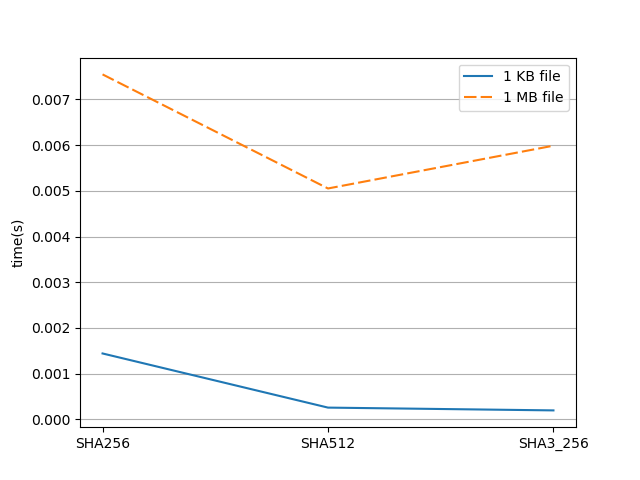
\includegraphics[scale=0.5]{q1d}
\end{figure}

Observation:
Comparing between two algorithm with same key size SHA3 256 and SHA 256

As from the lecture we know that hash functions needs to compute hash as fast as possible,eg.(If we have to check the integrity of the a 1TB hard disk it can not take ages to calculate the hash). From the above we can clearly see that SHA3 256 has had significant improvement to it, as compared to it prior. Which is one of the reasons which makes it a better algorithm for hashing to use.
 
Comparing between same algorithm with different key size SHA 256 and SHA 512

Here is a very interesting observation, as one will expect the time to compute hash must increase with the increase in the size. But we observe the opposite of it. As per my research this anomaly is because, our current laptops are 64 bit processor, because of which SHA 512 takes lesser cycles per byte of data, hence this improves its performance in 64 bit machines.

\subsection{Solution (e)}
\begin{lstlisting}[language=Python]
from Crypto.PublicKey import RSA
from Crypto.Cipher import PKCS1_OAEP
from Crypto import Random
import os, struct
import matplotlib.pyplot as plt
from timeit import default_timer as timer

start_key=timer()
random_generator = Random.new().read
keys = RSA.generate(2048, random_generator)
end_key=timer()

def get_time_per_byte(capture_time):
    return [capture_time[0]/(1024*1024), capture_time[1]/(1024*1024),
            capture_time[2]/(1024),capture_time[3]/(1024)]

with open('id_rsa2048', 'wb') as fin:
    fin.write(keys.export_key('PEM'))
with open('id_rsa2048.pub', 'wb') as fin:
    fin.write(keys.publickey().exportKey("PEM") )

def encrypt(input_file, enc_file):
    t_time=0
    pub_key = RSA.importKey(open('id_rsa2048.pub').read())
    cipher = PKCS1_OAEP.new(pub_key)
    size = 214
    file_size = os.path.getsize(input_file)
    with open(enc_file, 'wb') as fout:
        with open(input_file, 'rb') as fin:
            while True:
                data = fin.read(size)
                if len(data)==0:
                    break
                start = timer()
                encd = cipher.encrypt(data)
                end = timer()
                t_time+=(end-start)
                fout.write(encd)
    return t_time
def decrypt(enc_file, verification_file):
    t_time=0
    priavte_key = RSA.importKey(open('id_rsa2048').read())
    with open(enc_file, 'rb') as fin:
        cipher = PKCS1_OAEP.new(priavte_key)
        with open(verification_file, 'wb') as fout:
            while True:
                data = fin.read(256)
                if len(data) == 0:
                    break
                start = timer()
                pt=cipher.decrypt(data)
                end = timer()
                t_time+=(end-start)
                fout.write(pt)
    return t_time

input_files=['bigfile.txt', 'smallfile.txt']
enc_files=['q1eAnsBigFile.enc', 'q1eAnsSmallFile.enc']
verification_files=['q1eVeriBigFile.txt', 'q1eVeriSmallFile.enc']
capture_time=[]
for i in range(2):
    capture_time.append(encrypt(input_files[i], enc_files[i]))
    capture_time.append(decrypt(enc_files[i], verification_files[i]))

plt.plot(capture_time[:2], label='1 MB file')
plt.plot(capture_time[2:4], dashes=[6, 2], label='1 KB file')
plt.xticks(range(2), ['Encryption','Decryption'])
plt.ylabel('time(s)')
plt.grid(axis='y', linestyle='-')
plt.legend()
plt.savefig('q1e.png')
time_per_byte=get_time_per_byte(capture_time)
print('Total time')
print('Encryption -  1MB: %E, 1KB: %E' %(capture_time[0], capture_time[2]))
print('Decryption -  1MB: %E, 1KB: %E' %(capture_time[1], capture_time[3]))
print('Per Byte')
print('Encryption -  1MB: %E, 1KB: %E' %(time_per_byte[0], time_per_byte[2]))
print('Decryption -  1MB: %E, 1KB: %E' %(time_per_byte[1], time_per_byte[3]))
print('Key Gen')
print('Time: %E' %(end_key-start_key))

\end{lstlisting}

\begin{tabular}{ |p{8cm}|p{3cm}|p{3cm}|p{3cm} }
 \hline
 \multicolumn{3}{|c|}{RSA 2048} \\
 \hline
	 & 1MB file & 1KB file\\
 \hline
 Time taken for full file Encryption   & 4.229324E+00     &7.382428E-03   \\
  \hline
 Time taken for full file Decryption & 1.308226E+01   & 	1.259474E-02\\
 \hline
 Time taken per byte Encryption   & 4.033398E-06     & 7.209402E-06  \\
  \hline
 Time taken per byte Decryption & 1.247621E-05   &1.229955E-05 	\\
 \hline
 Time taken for key generation &  1.433346E-01  & 	\\
 \hline
\end{tabular}
\begin{figure}[h]
    \centering
	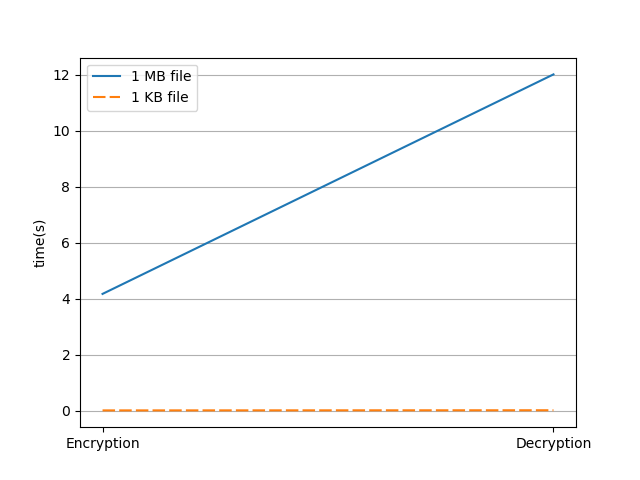
\includegraphics[scale=0.5]{q1e}
\end{figure}

Observation:
Two important expected behaviours:

We can observe that decryption takes significantly more time than encryption, reason being that data is encrypted with the public key, and decrypt using private key. As we already know that the computation involving private key will be costlier than public key as the private has a larger prime number. Behaves as expected.

In general we can observe a huge increase in the encryption and decryption compared to AES(Symmetrical Encryption). From the lectures we know that RSA is not suitable for encryption which involves larger file size than key, mostly RSA is used with very short message. For encrypting a large file with RSA, we have to sequentially encrypted our file (That is break our file into smaller chunks eg, 256 bit), and then encrypt each block with a huge key, this  is the reason for the huge difference. Main reason for RSA to be slow is that it involves calculation of modular exponentiation operation.

Additional observation is that the file size of the encrypted file increased more than the actual file. Reason for this increase in the file size can be related to 214 block size and not 256. Over every iteration (256-214) bit gets added more than the message. Hence this leads to the increase in the size.

\begin{figure}[h]
    \centering
	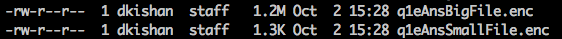
\includegraphics[scale=0.5]{4}
\end{figure}

\subsection{Solution (f)}
\begin{lstlisting}[language=Python]
from Crypto.PublicKey import RSA
from Crypto.Cipher import PKCS1_OAEP
from Crypto import Random
import os, struct
import matplotlib.pyplot as plt
from timeit import default_timer as timer

start_key=timer()
random_generator = Random.new().read
keys = RSA.generate(3072, random_generator)
end_key=timer()

def get_time_per_byte(capture_time):
    return [capture_time[0]/(1024*1024), capture_time[1]/(1024*1024),
            capture_time[2]/(1024),capture_time[3]/(1024)]

with open('id_rsa3072', 'wb') as fin:
    fin.write(keys.export_key('PEM'))
with open('id_rsa3072.pub', 'wb') as fin:
    fin.write(keys.publickey().exportKey("PEM") )

def encrypt(input_file, enc_file):
    t_time=0
    pub_key = RSA.importKey(open('id_rsa3072.pub').read())
    cipher = PKCS1_OAEP.new(pub_key)
    size = 342
    file_size = os.path.getsize(input_file)
    with open(enc_file, 'wb') as fout:
        with open(input_file, 'rb') as fin:
            while True:
                data = fin.read(size)
                if len(data)==0:
                    break
                start = timer()
                encd = cipher.encrypt(data)
                end = timer()
                t_time+=(end-start)
                fout.write(encd)
    return t_time
def decrypt(enc_file, verification_file):
    t_time=0
    priavte_key = RSA.importKey(open('id_rsa3072').read())
    with open(enc_file, 'rb') as fin:
        cipher = PKCS1_OAEP.new(priavte_key)
        with open(verification_file, 'wb') as fout:
            while True:
                data = fin.read(384)
                if len(data) == 0:
                    break
                start = timer()
                pt=cipher.decrypt(data)
                end = timer()
                t_time+=(end-start)
                fout.write(pt)
    return t_time

input_files=['bigfile.txt', 'smallfile.txt']
enc_files=['q1fAnsBigFile.enc', 'q1fAnsSmallFile.enc']
verification_files=['q1fVeriBigFile.txt', 'q1fVeriSmallFile.enc']
capture_time=[]
for i in range(2):
    capture_time.append(encrypt(input_files[i], enc_files[i]))
    capture_time.append(decrypt(enc_files[i], verification_files[i]))

plt.plot(capture_time[:2], label='1 MB file')
plt.plot(capture_time[2:4], dashes=[6, 2], label='1 KB file')
plt.xticks(range(2), ['Encryption','Decryption'])
plt.ylabel('time(s)')
plt.grid(axis='y', linestyle='-')
plt.legend()
plt.savefig('q1f.png')
time_per_byte=get_time_per_byte(capture_time)
print('Total time')
print('Encryption -  1MB: %E, 1KB: %E' %(capture_time[0], capture_time[2]))
print('Decryption -  1MB: %E, 1KB: %E' %(capture_time[1], capture_time[3]))
print('Per Byte')
print('Encryption -  1MB: %E, 1KB: %E' %(time_per_byte[0], time_per_byte[2]))
print('Decryption -  1MB: %E, 1KB: %E' %(time_per_byte[1], time_per_byte[3]))
print('Key Gen')
print('Time: %E' %(end_key-start_key))

\end{lstlisting}
\begin{tabular}{ |p{8cm}|p{3cm}|p{3cm}|p{3cm} }
 \hline
 \multicolumn{3}{|c|}{RSA 3072} \\
 \hline
	 & 1MB file & 1KB file\\
 \hline
 Time taken for full file Encryption   &  5.198703E+00    &  5.419426E-03 \\
  \hline
 Time taken for full file Decryption & 1.852010E+01   & 1.719529E-02	\\
 \hline
 Time taken per byte Encryption   &   4.957869E-06   &  5.292408E-06 \\
  \hline
 Time taken per byte Decryption & 1.766214E-05   & 1.679228E-05	\\
 \hline
 Time taken for key generation & 9.007486E-01   & 	\\
 \hline
\end{tabular}

\begin{figure}[h]
    \centering
	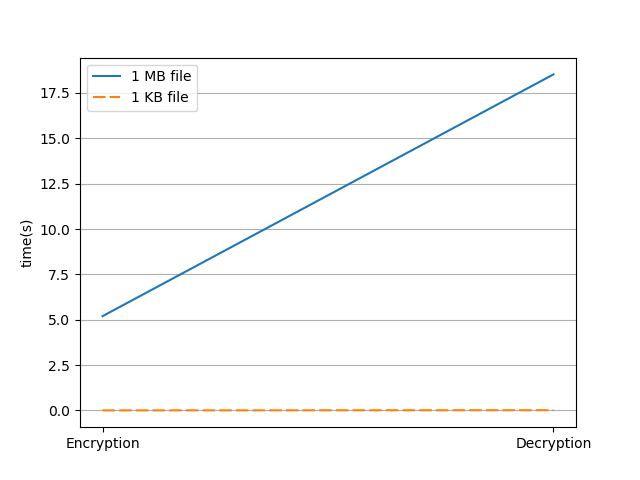
\includegraphics[scale=0.5]{q1f}
\end{figure}

Observation:
RSA(3072) as expected has a higher key generation, encryption and decryption time than RSA(2048), same reason more computation gets costlier with bigger key.

\subsection{Solution (g)}
\begin{lstlisting}[language=Python]
from cryptography.hazmat.backends import default_backend
from cryptography.hazmat.primitives import hashes
from cryptography.hazmat.primitives.asymmetric import dsa
from cryptography.hazmat.primitives.asymmetric import utils
import matplotlib.pyplot as plt
from timeit import default_timer as timer
start_key=timer()
private_key = dsa.generate_private_key(
    key_size=2048,
    backend=default_backend()
)
end_key=timer()

def sign(digest, chosen_hash):
    return private_key.sign(digest, utils.Prehashed(chosen_hash))

def verify(signature, digest, chosen_hash):
    try:
        public_key = private_key.public_key()
        public_key.verify(signature, digest, utils.Prehashed(chosen_hash))
        return True
    except:
        return False
capture_time=[]
for file in ['bigfile.txt', 'smallfile.txt']:
    chosen_hash = hashes.SHA256()
    hasher = hashes.Hash(chosen_hash, default_backend())
    hasher.update(open(file, 'rb').read())
    digest = hasher.finalize()
    start = timer()
    signature = sign(digest, chosen_hash)
    end = timer()
    capture_time.append(end-start)
    start = timer()
    check=verify(signature, digest, chosen_hash)
    end = timer()
    capture_time.append(end-start)
    if check:
        print('Verification successfull')
    else:
        print('Verification failed')
plt.plot(capture_time[:2], label='1 MB file')
plt.plot(capture_time[2:4], dashes=[6, 2], label='1 KB file')
plt.xticks(range(2), ['Sign','Verify'])
plt.ylabel('time(s)')
plt.grid(axis='y', linestyle='-')
plt.legend()
plt.savefig('q1g.png')
print('Total time')
print('Signing -  1MB: %E, 1KB: %E' %(capture_time[0], capture_time[2]))
print('Verification -  1MB: %E, 1KB: %E' %(capture_time[1], capture_time[3]))
print('Key Gen')
print('Time: %E' %(end_key-start_key))

\end{lstlisting}
\begin{tabular}{ |p{8cm}|p{3cm}|p{3cm}|p{3cm} }
 \hline
 \multicolumn{3}{|c|}{DSA 2048} \\
 \hline
	 & 1MB file & 1KB file\\
 \hline
 Time taken for signing  &   1.184230E-03   &  1.046116E-03 \\
  \hline
 Time taken for verification &   1.044038E-03 & 	1.027338E-03\\
 \hline
 Time taken for key generation & 3.895689E-01   & 	\\
 \hline
\end{tabular}

\begin{figure}[h]
    \centering
	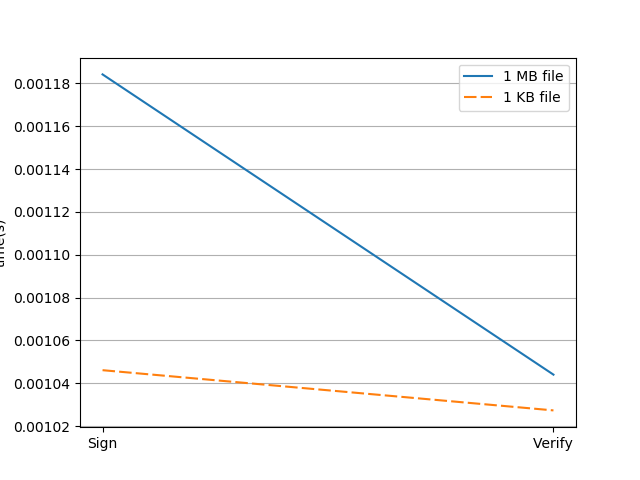
\includegraphics[scale=0.5]{q1g}
\end{figure}

Observation: 
It can be observed that signing the key takes more time compared to verification as private key is being used for signing and verification public key is used. This is also a expected behaviour (modular exponentiation operation). 


\subsection{Solution (h)}
\begin{lstlisting}[language=Python]
from cryptography.hazmat.backends import default_backend
from cryptography.hazmat.primitives import hashes
from cryptography.hazmat.primitives.asymmetric import dsa
from cryptography.hazmat.primitives.asymmetric import utils
import matplotlib.pyplot as plt
from timeit import default_timer as timer
start_key=timer()
private_key = dsa.generate_private_key(
    key_size=3072,
    backend=default_backend()
)
end_key=timer()

def sign(digest, chosen_hash):
    return private_key.sign(digest, utils.Prehashed(chosen_hash))

def verify(signature, digest, chosen_hash):
    try:
        public_key = private_key.public_key()
        public_key.verify(signature, digest, utils.Prehashed(chosen_hash))
        return True
    except:
        return False
capture_time=[]
for file in ['bigfile.txt', 'smallfile.txt']:
    chosen_hash = hashes.SHA256()
    hasher = hashes.Hash(chosen_hash, default_backend())
    hasher.update(open(file, 'rb').read())
    digest = hasher.finalize()
    start = timer()
    signature = sign(digest, chosen_hash)
    end = timer()
    capture_time.append(end-start)
    start = timer()
    check=verify(signature, digest, chosen_hash)
    end = timer()
    capture_time.append(end-start)
    if check:
        print('Verification successfull')
    else:
        print('Verification failed')
plt.plot(capture_time[:2], label='1 MB file')
plt.plot(capture_time[2:4], dashes=[6, 2], label='1 KB file')
plt.xticks(range(2), ['Sign','Verify'])
plt.ylabel('time(s)')
plt.grid(axis='y', linestyle='-')
plt.legend()
plt.savefig('q1h.png')
print('Total time')
print('Signing -  1MB: %E, 1KB: %E' %(capture_time[0], capture_time[2]))
print('Verification -  1MB: %E, 1KB: %E' %(capture_time[1], capture_time[3]))
print('Key Gen')
print('Time: %E' %(end_key-start_key))

\end{lstlisting}
\begin{tabular}{ |p{8cm}|p{3cm}|p{3cm}|p{3cm} }
 \hline
 \multicolumn{3}{|c|}{DSA 3072} \\
 \hline
	 & 1MB file & 1KB file\\
 \hline
 Time taken for signing  &   2.762864E-03   &  1.789431E-03 \\
  \hline
 Time taken for verification &   2.693177E-03 & 	1.732421E-03\\
 \hline
 Time taken for key generation & 2.651182E+00   & 	\\
 \hline
\end{tabular}
\begin{figure}[h]
    \centering
	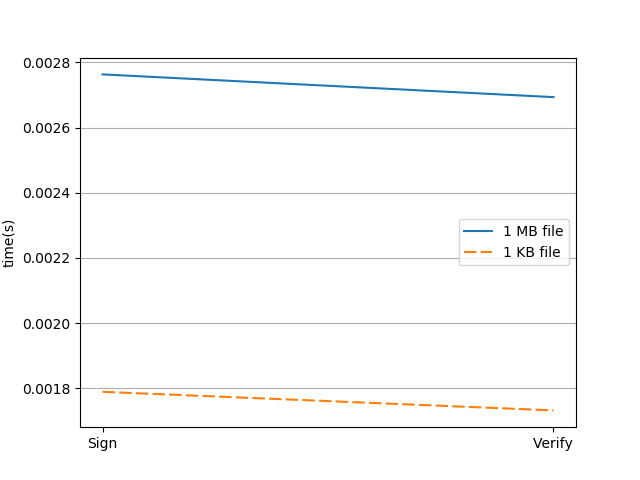
\includegraphics[scale=0.5]{q1h}
\end{figure}

Observation: 
Longer the key length, more time for key generation, signing and verification as compared with DSA 2048. 

\section{Problem 2}
\subsection{Solution (a)}
\[if ( modify \in A_i[S_1, o]\quad \textrm{and} \quad modify \in A_i[S_1, S_2] \quad \textrm{and}\quad own \notin A_i[S_2,o])\quad then;\]
\[A_{i+1} = A_i\]
\[A_{i+1} [S_2, o] = \emptyset\]
\subsection{Solution (b)}

Let r' is the set of copy/grant rights which S\_1 has over object 0

\[R^* = \{ r^* , w^*, e^*, a^*, l^*, m^* \}\]
 \[r'\quad = \quad A_i[S_1,0] \quad \cap \quad	R^*\]
 Let \[\quad C = \quad \emptyset\]
 \[if(  r^* \in r' \quad and \quad r\notin A_i[S_2, o] ); then\]
 \[\quad C = C \cup \{r\}\]
\[if(  w^* \in r' and \quad w \notin A_i[S_2, o] ); then\]
 \[\quad C = C \cup \{w\}\]
\[if(  e^* \in r' and \quad e \notin A_i[S_2, o]); then\]
 \[\quad C = C \cup \{e\}\]
\[if(  a^* \in r' and \quad a \notin A_i[S_2, o]); then\]
 \[\quad C = C \cup \{a\}\]
\[if(  l^* \in r' and \quad l \notin A_i[S_2, o]); then\]
 \[\quad C = C \cup \{l\}\]
 \[if(  m^* \in r' and \quad m \notin A_i[S_2, o]); then\]
 \[\quad C = C \cup \{m\}\]
 
  \[A_{i+1}[S_2,o]=A_i[S_2,o] \cup C\]
\end{document}
              
            
